\documentclass[twoside]{book}

% Packages required by doxygen
\usepackage{calc}
\usepackage{doxygen}
\usepackage{graphicx}
\usepackage[utf8]{inputenc}
\usepackage{makeidx}
\usepackage{multicol}
\usepackage{multirow}
\usepackage{textcomp}
\usepackage[table]{xcolor}

% Font selection
\usepackage[T1]{fontenc}
\usepackage{mathptmx}
\usepackage[scaled=.90]{helvet}
\usepackage{courier}
\usepackage{amssymb}
\usepackage{sectsty}
\renewcommand{\familydefault}{\sfdefault}
\allsectionsfont{%
  \fontseries{bc}\selectfont%
  \color{darkgray}%
}
\renewcommand{\DoxyLabelFont}{%
  \fontseries{bc}\selectfont%
  \color{darkgray}%
}

% Page & text layout
\usepackage{geometry}
\geometry{%
  a4paper,%
  top=2.5cm,%
  bottom=2.5cm,%
  left=2.5cm,%
  right=2.5cm%
}
\tolerance=750
\hfuzz=15pt
\hbadness=750
\setlength{\emergencystretch}{15pt}
\setlength{\parindent}{0cm}
\setlength{\parskip}{0.2cm}
\makeatletter
\renewcommand{\paragraph}{%
  \@startsection{paragraph}{4}{0ex}{-1.0ex}{1.0ex}{%
    \normalfont\normalsize\bfseries\SS@parafont%
  }%
}
\renewcommand{\subparagraph}{%
  \@startsection{subparagraph}{5}{0ex}{-1.0ex}{1.0ex}{%
    \normalfont\normalsize\bfseries\SS@subparafont%
  }%
}
\makeatother

% Headers & footers
\usepackage{fancyhdr}
\pagestyle{fancyplain}
\fancyhead[LE]{\fancyplain{}{\bfseries\thepage}}
\fancyhead[CE]{\fancyplain{}{}}
\fancyhead[RE]{\fancyplain{}{\bfseries\leftmark}}
\fancyhead[LO]{\fancyplain{}{\bfseries\rightmark}}
\fancyhead[CO]{\fancyplain{}{}}
\fancyhead[RO]{\fancyplain{}{\bfseries\thepage}}
\fancyfoot[LE]{\fancyplain{}{}}
\fancyfoot[CE]{\fancyplain{}{}}
\fancyfoot[RE]{\fancyplain{}{\bfseries\scriptsize Generated on Mon Jan 6 2020 17\-:38\-:37 for My Project by Doxygen }}
\fancyfoot[LO]{\fancyplain{}{\bfseries\scriptsize Generated on Mon Jan 6 2020 17\-:38\-:37 for My Project by Doxygen }}
\fancyfoot[CO]{\fancyplain{}{}}
\fancyfoot[RO]{\fancyplain{}{}}
\renewcommand{\footrulewidth}{0.4pt}
\renewcommand{\chaptermark}[1]{%
  \markboth{#1}{}%
}
\renewcommand{\sectionmark}[1]{%
  \markright{\thesection\ #1}%
}

% Indices & bibliography
\usepackage{natbib}
\usepackage[titles]{tocloft}
\setcounter{tocdepth}{3}
\setcounter{secnumdepth}{5}
\makeindex

% Hyperlinks (required, but should be loaded last)
\usepackage{ifpdf}
\ifpdf
  \usepackage[pdftex,pagebackref=true]{hyperref}
\else
  \usepackage[ps2pdf,pagebackref=true]{hyperref}
\fi
\hypersetup{%
  colorlinks=true,%
  linkcolor=blue,%
  citecolor=blue,%
  unicode%
}

% Custom commands
\newcommand{\clearemptydoublepage}{%
  \newpage{\pagestyle{empty}\cleardoublepage}%
}


%===== C O N T E N T S =====

\begin{document}

% Titlepage & ToC
\hypersetup{pageanchor=false}
\pagenumbering{roman}
\begin{titlepage}
\vspace*{7cm}
\begin{center}%
{\Large My Project }\\
\vspace*{1cm}
{\large Generated by Doxygen 1.8.5}\\
\vspace*{0.5cm}
{\small Mon Jan 6 2020 17:38:37}\\
\end{center}
\end{titlepage}
\clearemptydoublepage
\tableofcontents
\clearemptydoublepage
\pagenumbering{arabic}
\hypersetup{pageanchor=true}

%--- Begin generated contents ---
\chapter{pic}
\label{md_README}
\hypertarget{md_README}{}
\input{md_README}
\chapter{Namespace Index}
\section{Namespace List}
Here is a list of all documented namespaces with brief descriptions\-:\begin{DoxyCompactList}
\item\contentsline{section}{\hyperlink{namespaceGrid}{Grid} }{\pageref{namespaceGrid}}{}
\item\contentsline{section}{\hyperlink{namespaceGrid1D}{Grid1\-D} }{\pageref{namespaceGrid1D}}{}
\item\contentsline{section}{\hyperlink{namespaceGrid1DCartesian}{Grid1\-D\-Cartesian} }{\pageref{namespaceGrid1DCartesian}}{}
\item\contentsline{section}{\hyperlink{namespaceShape}{Shape} }{\pageref{namespaceShape}}{}
\item\contentsline{section}{\hyperlink{namespaceShape1D}{Shape1\-D} }{\pageref{namespaceShape1D}}{}
\item\contentsline{section}{\hyperlink{namespaceShape1DTriangle}{Shape1\-D\-Triangle} }{\pageref{namespaceShape1DTriangle}}{}
\end{DoxyCompactList}

\chapter{Hierarchical Index}
\section{Class Hierarchy}
This inheritance list is sorted roughly, but not completely, alphabetically\-:\begin{DoxyCompactList}
\item \contentsline{section}{Grid.\-Grid}{\pageref{classGrid_1_1Grid}}{}
\begin{DoxyCompactList}
\item \contentsline{section}{Grid1\-D.\-Grid1\-D}{\pageref{classGrid1D_1_1Grid1D}}{}
\begin{DoxyCompactList}
\item \contentsline{section}{Grid1\-D\-Cartesian.\-Grid1\-D\-Cartesian}{\pageref{classGrid1DCartesian_1_1Grid1DCartesian}}{}
\end{DoxyCompactList}
\end{DoxyCompactList}
\item \contentsline{section}{Shape.\-Shape}{\pageref{classShape_1_1Shape}}{}
\begin{DoxyCompactList}
\item \contentsline{section}{Shape1\-D.\-Shape1\-D}{\pageref{classShape1D_1_1Shape1D}}{}
\begin{DoxyCompactList}
\item \contentsline{section}{Shape1\-D\-Triangle.\-Shape1\-D\-Triangle}{\pageref{classShape1DTriangle_1_1Shape1DTriangle}}{}
\end{DoxyCompactList}
\end{DoxyCompactList}
\end{DoxyCompactList}

\chapter{Class Index}
\section{Class List}
Here are the classes, structs, unions and interfaces with brief descriptions\-:\begin{DoxyCompactList}
\item\contentsline{section}{\hyperlink{classGrid_1_1Grid}{Grid.\-Grid} }{\pageref{classGrid_1_1Grid}}{}
\item\contentsline{section}{\hyperlink{classGrid1D_1_1Grid1D}{Grid1\-D.\-Grid1\-D} }{\pageref{classGrid1D_1_1Grid1D}}{}
\item\contentsline{section}{\hyperlink{classGrid1DCartesian_1_1Grid1DCartesian}{Grid1\-D\-Cartesian.\-Grid1\-D\-Cartesian} }{\pageref{classGrid1DCartesian_1_1Grid1DCartesian}}{}
\item\contentsline{section}{\hyperlink{classShape_1_1Shape}{Shape.\-Shape} }{\pageref{classShape_1_1Shape}}{}
\item\contentsline{section}{\hyperlink{classShape1D_1_1Shape1D}{Shape1\-D.\-Shape1\-D} }{\pageref{classShape1D_1_1Shape1D}}{}
\item\contentsline{section}{\hyperlink{classShape1DTriangle_1_1Shape1DTriangle}{Shape1\-D\-Triangle.\-Shape1\-D\-Triangle} }{\pageref{classShape1DTriangle_1_1Shape1DTriangle}}{}
\end{DoxyCompactList}

\chapter{Namespace Documentation}
\hypertarget{namespaceGrid}{\section{Grid Namespace Reference}
\label{namespaceGrid}\index{Grid@{Grid}}
}
\subsection*{Classes}
\begin{DoxyCompactItemize}
\item 
class \hyperlink{classGrid_1_1Grid}{Grid}
\end{DoxyCompactItemize}


\subsection{Detailed Description}
\begin{DoxyVerb}@package Grid.py
Documentation for Grid class (ABC)
\end{DoxyVerb}
 
\hypertarget{namespaceGrid1D}{\section{Grid1\-D Namespace Reference}
\label{namespaceGrid1D}\index{Grid1\-D@{Grid1\-D}}
}
\subsection*{Classes}
\begin{DoxyCompactItemize}
\item 
class \hyperlink{classGrid1D_1_1Grid1D}{Grid1\-D}
\end{DoxyCompactItemize}


\subsection{Detailed Description}
\begin{DoxyVerb}@package Grid1D.py
Documentation for Grid1D class (ABC)
\end{DoxyVerb}
 
\hypertarget{namespaceGrid1DCartesian}{\section{Grid1\-D\-Cartesian Namespace Reference}
\label{namespaceGrid1DCartesian}\index{Grid1\-D\-Cartesian@{Grid1\-D\-Cartesian}}
}
\subsection*{Classes}
\begin{DoxyCompactItemize}
\item 
class \hyperlink{classGrid1DCartesian_1_1Grid1DCartesian}{Grid1\-D\-Cartesian}
\end{DoxyCompactItemize}


\subsection{Detailed Description}
\begin{DoxyVerb}@package Grid1DCartesian.py
Documentation for Grid1DCartesian class
\end{DoxyVerb}
 
\hypertarget{namespaceShape}{\section{Shape Namespace Reference}
\label{namespaceShape}\index{Shape@{Shape}}
}
\subsection*{Classes}
\begin{DoxyCompactItemize}
\item 
class \hyperlink{classShape_1_1Shape}{Shape}
\end{DoxyCompactItemize}


\subsection{Detailed Description}
\begin{DoxyVerb}@package Shape.py
Documentation for Shape class (ABC)
\end{DoxyVerb}
 
\hypertarget{namespaceShape1D}{\section{Shape1\-D Namespace Reference}
\label{namespaceShape1D}\index{Shape1\-D@{Shape1\-D}}
}
\subsection*{Classes}
\begin{DoxyCompactItemize}
\item 
class \hyperlink{classShape1D_1_1Shape1D}{Shape1\-D}
\end{DoxyCompactItemize}


\subsection{Detailed Description}
\begin{DoxyVerb}@package Shape1D.py
Documentation for Shape1D class (ABC)
\end{DoxyVerb}
 
\hypertarget{namespaceShape1DTriangle}{\section{Shape1\-D\-Triangle Namespace Reference}
\label{namespaceShape1DTriangle}\index{Shape1\-D\-Triangle@{Shape1\-D\-Triangle}}
}
\subsection*{Classes}
\begin{DoxyCompactItemize}
\item 
class \hyperlink{classShape1DTriangle_1_1Shape1DTriangle}{Shape1\-D\-Triangle}
\end{DoxyCompactItemize}


\subsection{Detailed Description}
\begin{DoxyVerb}@package Shape1DTrangle.py
Documentation for Shape1DTrangle class
\end{DoxyVerb}
 
\chapter{Class Documentation}
\hypertarget{classGrid_1_1Grid}{\section{Grid.\-Grid Class Reference}
\label{classGrid_1_1Grid}\index{Grid.\-Grid@{Grid.\-Grid}}
}
Inheritance diagram for Grid.\-Grid\-:\begin{figure}[H]
\begin{center}
\leavevmode
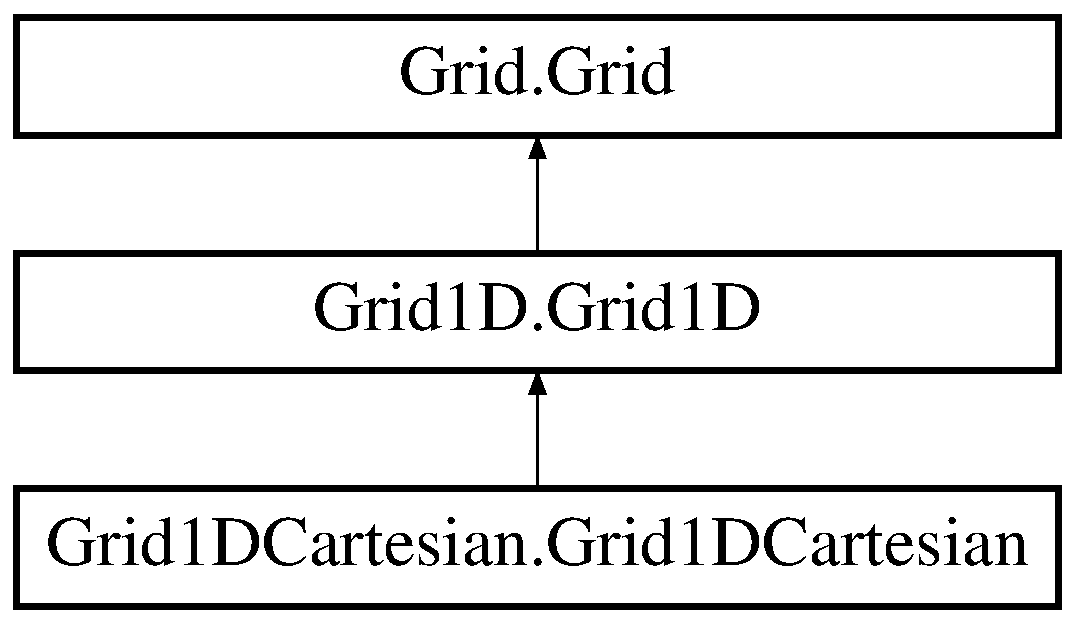
\includegraphics[height=3.000000cm]{classGrid_1_1Grid}
\end{center}
\end{figure}
\subsection*{Public Member Functions}
\begin{DoxyCompactItemize}
\item 
def \hyperlink{classGrid_1_1Grid_acbb39beb7e85435989317b14ac7000a6}{\-\_\-\-\_\-init\-\_\-\-\_\-}
\item 
def \hyperlink{classGrid_1_1Grid_aede8950228046ba7d946279b5dcb62d6}{set\-\_\-grid\-\_\-container}
\end{DoxyCompactItemize}


\subsection{Detailed Description}
\begin{DoxyVerb}Documentation for Grid class.
\end{DoxyVerb}
 

\subsection{Constructor \& Destructor Documentation}
\hypertarget{classGrid_1_1Grid_acbb39beb7e85435989317b14ac7000a6}{\index{Grid\-::\-Grid@{Grid\-::\-Grid}!\-\_\-\-\_\-init\-\_\-\-\_\-@{\-\_\-\-\_\-init\-\_\-\-\_\-}}
\index{\-\_\-\-\_\-init\-\_\-\-\_\-@{\-\_\-\-\_\-init\-\_\-\-\_\-}!Grid::Grid@{Grid\-::\-Grid}}
\subsubsection[{\-\_\-\-\_\-init\-\_\-\-\_\-}]{\setlength{\rightskip}{0pt plus 5cm}def Grid.\-Grid.\-\_\-\-\_\-init\-\_\-\-\_\- (
\begin{DoxyParamCaption}
\item[{}]{self, }
\item[{}]{grid\-\_\-step, }
\item[{}]{grid\-\_\-size}
\end{DoxyParamCaption}
)}}\label{classGrid_1_1Grid_acbb39beb7e85435989317b14ac7000a6}
\begin{DoxyVerb}The constructor
\end{DoxyVerb}
 

\subsection{Member Function Documentation}
\hypertarget{classGrid_1_1Grid_aede8950228046ba7d946279b5dcb62d6}{\index{Grid\-::\-Grid@{Grid\-::\-Grid}!set\-\_\-grid\-\_\-container@{set\-\_\-grid\-\_\-container}}
\index{set\-\_\-grid\-\_\-container@{set\-\_\-grid\-\_\-container}!Grid::Grid@{Grid\-::\-Grid}}
\subsubsection[{set\-\_\-grid\-\_\-container}]{\setlength{\rightskip}{0pt plus 5cm}def Grid.\-Grid.\-set\-\_\-grid\-\_\-container (
\begin{DoxyParamCaption}
\item[{}]{self, }
\item[{}]{grid, }
\item[{}]{is\-\_\-shifted, }
\item[{}]{grid\-\_\-container}
\end{DoxyParamCaption}
)}}\label{classGrid_1_1Grid_aede8950228046ba7d946279b5dcb62d6}
\begin{DoxyVerb}Setting values of grid container (i.e. fields or sources)
\end{DoxyVerb}
 

The documentation for this class was generated from the following file\-:\begin{DoxyCompactItemize}
\item 
Grid.\-py\end{DoxyCompactItemize}

\hypertarget{classGrid1D_1_1Grid1D}{\section{Grid1\-D.\-Grid1\-D Class Reference}
\label{classGrid1D_1_1Grid1D}\index{Grid1\-D.\-Grid1\-D@{Grid1\-D.\-Grid1\-D}}
}
Inheritance diagram for Grid1\-D.\-Grid1\-D\-:\begin{figure}[H]
\begin{center}
\leavevmode
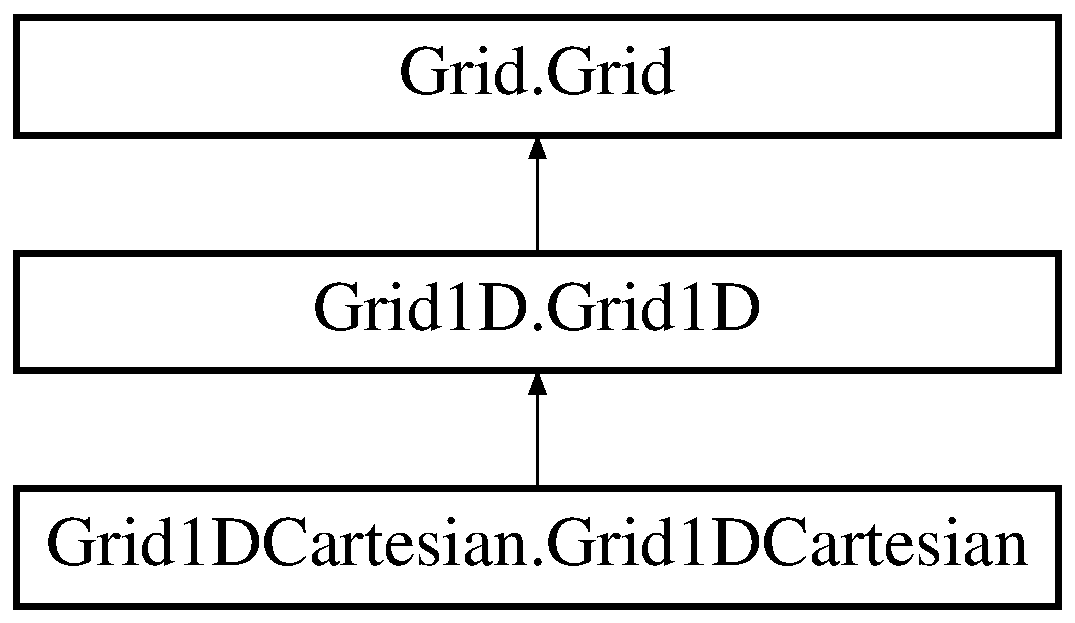
\includegraphics[height=3.000000cm]{classGrid1D_1_1Grid1D}
\end{center}
\end{figure}
\subsection*{Additional Inherited Members}


\subsection{Detailed Description}
\begin{DoxyVerb}Documentation for Grid1D class
\end{DoxyVerb}
 

The documentation for this class was generated from the following file\-:\begin{DoxyCompactItemize}
\item 
Grid1\-D.\-py\end{DoxyCompactItemize}

\hypertarget{classGrid1DCartesian_1_1Grid1DCartesian}{\section{Grid1\-D\-Cartesian.\-Grid1\-D\-Cartesian Class Reference}
\label{classGrid1DCartesian_1_1Grid1DCartesian}\index{Grid1\-D\-Cartesian.\-Grid1\-D\-Cartesian@{Grid1\-D\-Cartesian.\-Grid1\-D\-Cartesian}}
}
Inheritance diagram for Grid1\-D\-Cartesian.\-Grid1\-D\-Cartesian\-:\begin{figure}[H]
\begin{center}
\leavevmode
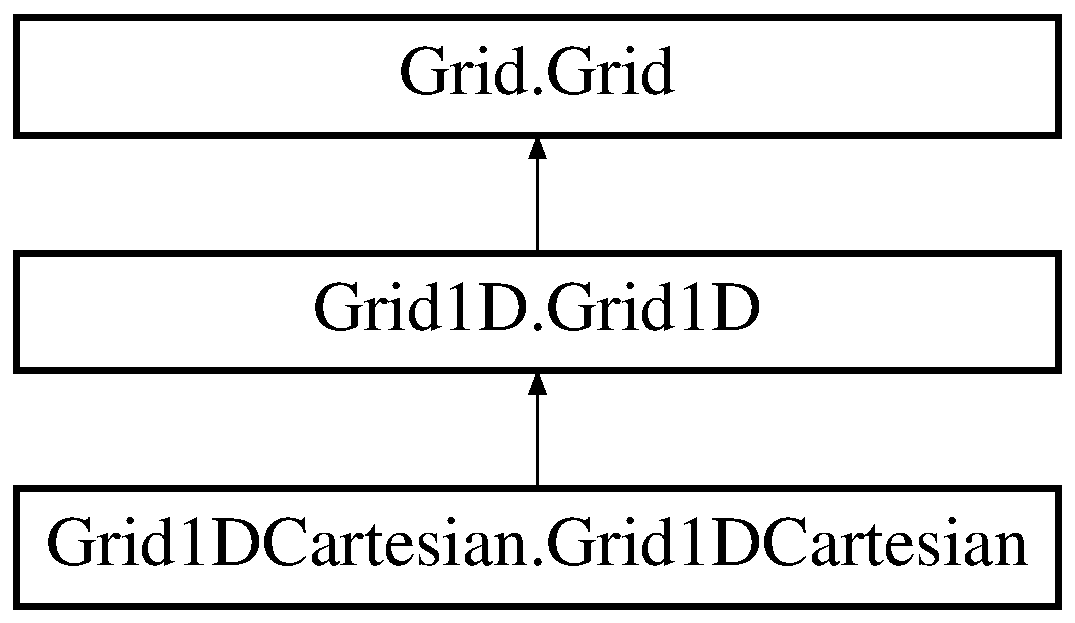
\includegraphics[height=3.000000cm]{classGrid1DCartesian_1_1Grid1DCartesian}
\end{center}
\end{figure}
\subsection*{Public Member Functions}
\begin{DoxyCompactItemize}
\item 
def \hyperlink{classGrid1DCartesian_1_1Grid1DCartesian_a7aa69514393f49e62b5b6e52474bba66}{set\-\_\-grid}
\item 
def \hyperlink{classGrid1DCartesian_1_1Grid1DCartesian_ab65433172dcaf48d7e5b70bf8efe0c6f}{set\-\_\-grid\-\_\-container}
\item 
def \hyperlink{classGrid1DCartesian_1_1Grid1DCartesian_a54f1f22b80717d8f6a809a6a9f3c649b}{get\-\_\-grid\-\_\-container}
\end{DoxyCompactItemize}
\subsection*{Static Public Attributes}
\begin{DoxyCompactItemize}
\item 
\hypertarget{classGrid1DCartesian_1_1Grid1DCartesian_a9102b7faba7f5dc99f952e870d5149ea}{tuple {\bfseries Nx} = self.\-\_\-grid\-\_\-size.\-item(\-\_\-\-Ndims-\/1)}\label{classGrid1DCartesian_1_1Grid1DCartesian_a9102b7faba7f5dc99f952e870d5149ea}

\end{DoxyCompactItemize}


\subsection{Detailed Description}
\begin{DoxyVerb}Documentaiton for Grid1DCartesian class
\end{DoxyVerb}
 

\subsection{Member Function Documentation}
\hypertarget{classGrid1DCartesian_1_1Grid1DCartesian_a54f1f22b80717d8f6a809a6a9f3c649b}{\index{Grid1\-D\-Cartesian\-::\-Grid1\-D\-Cartesian@{Grid1\-D\-Cartesian\-::\-Grid1\-D\-Cartesian}!get\-\_\-grid\-\_\-container@{get\-\_\-grid\-\_\-container}}
\index{get\-\_\-grid\-\_\-container@{get\-\_\-grid\-\_\-container}!Grid1DCartesian::Grid1DCartesian@{Grid1\-D\-Cartesian\-::\-Grid1\-D\-Cartesian}}
\subsubsection[{get\-\_\-grid\-\_\-container}]{\setlength{\rightskip}{0pt plus 5cm}def Grid1\-D\-Cartesian.\-Grid1\-D\-Cartesian.\-get\-\_\-grid\-\_\-container (
\begin{DoxyParamCaption}
\item[{}]{self}
\end{DoxyParamCaption}
)}}\label{classGrid1DCartesian_1_1Grid1DCartesian_a54f1f22b80717d8f6a809a6a9f3c649b}
\begin{DoxyVerb}Accessing values of grid container (i.e. fields or sources)
\end{DoxyVerb}
 \hypertarget{classGrid1DCartesian_1_1Grid1DCartesian_a7aa69514393f49e62b5b6e52474bba66}{\index{Grid1\-D\-Cartesian\-::\-Grid1\-D\-Cartesian@{Grid1\-D\-Cartesian\-::\-Grid1\-D\-Cartesian}!set\-\_\-grid@{set\-\_\-grid}}
\index{set\-\_\-grid@{set\-\_\-grid}!Grid1DCartesian::Grid1DCartesian@{Grid1\-D\-Cartesian\-::\-Grid1\-D\-Cartesian}}
\subsubsection[{set\-\_\-grid}]{\setlength{\rightskip}{0pt plus 5cm}def Grid1\-D\-Cartesian.\-Grid1\-D\-Cartesian.\-set\-\_\-grid (
\begin{DoxyParamCaption}
\item[{}]{self}
\end{DoxyParamCaption}
)}}\label{classGrid1DCartesian_1_1Grid1DCartesian_a7aa69514393f49e62b5b6e52474bba66}
\begin{DoxyVerb}Set the grid after it is initialized
\end{DoxyVerb}
 \hypertarget{classGrid1DCartesian_1_1Grid1DCartesian_ab65433172dcaf48d7e5b70bf8efe0c6f}{\index{Grid1\-D\-Cartesian\-::\-Grid1\-D\-Cartesian@{Grid1\-D\-Cartesian\-::\-Grid1\-D\-Cartesian}!set\-\_\-grid\-\_\-container@{set\-\_\-grid\-\_\-container}}
\index{set\-\_\-grid\-\_\-container@{set\-\_\-grid\-\_\-container}!Grid1DCartesian::Grid1DCartesian@{Grid1\-D\-Cartesian\-::\-Grid1\-D\-Cartesian}}
\subsubsection[{set\-\_\-grid\-\_\-container}]{\setlength{\rightskip}{0pt plus 5cm}def Grid1\-D\-Cartesian.\-Grid1\-D\-Cartesian.\-set\-\_\-grid\-\_\-container (
\begin{DoxyParamCaption}
\item[{}]{self, }
\item[{}]{grid\-\_\-container}
\end{DoxyParamCaption}
)}}\label{classGrid1DCartesian_1_1Grid1DCartesian_ab65433172dcaf48d7e5b70bf8efe0c6f}
\begin{DoxyVerb}Setting values of grid container (i.e. fields or sources)
\end{DoxyVerb}
 

The documentation for this class was generated from the following file\-:\begin{DoxyCompactItemize}
\item 
Grid1\-D\-Cartesian.\-py\end{DoxyCompactItemize}

\hypertarget{classShape_1_1Shape}{\section{Shape.\-Shape Class Reference}
\label{classShape_1_1Shape}\index{Shape.\-Shape@{Shape.\-Shape}}
}
Inheritance diagram for Shape.\-Shape\-:\begin{figure}[H]
\begin{center}
\leavevmode
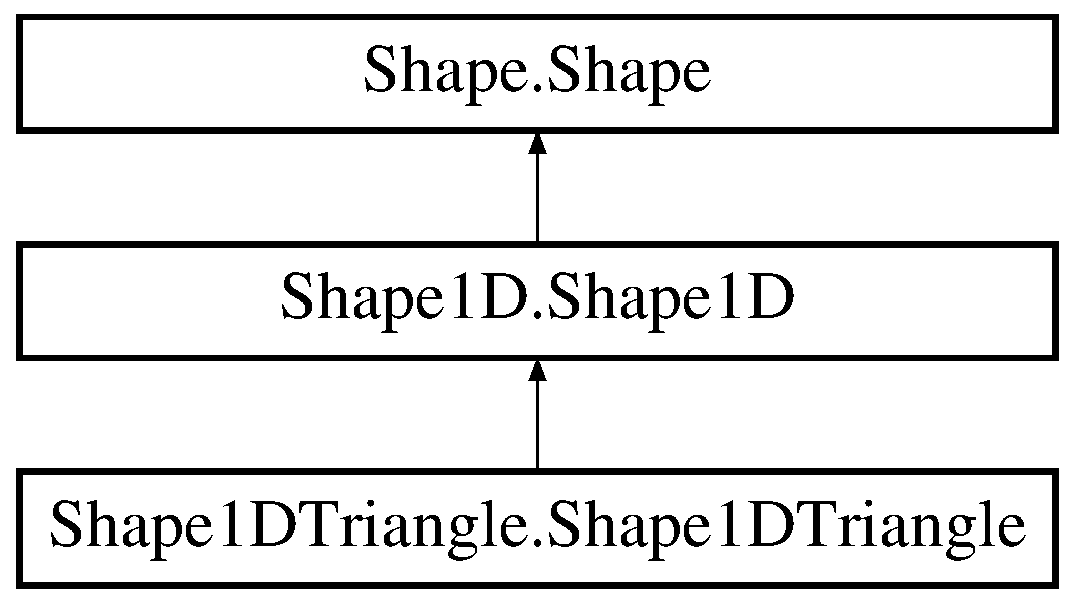
\includegraphics[height=3.000000cm]{classShape_1_1Shape}
\end{center}
\end{figure}
\subsection*{Public Member Functions}
\begin{DoxyCompactItemize}
\item 
def \hyperlink{classShape_1_1Shape_a24e8da4a47ca0ad94b99d51000e7fecd}{\-\_\-\-\_\-init\-\_\-\-\_\-}
\item 
def \hyperlink{classShape_1_1Shape_aa98535f2e48db66af771f4d4037b5e14}{set\-\_\-shape}
\item 
def \hyperlink{classShape_1_1Shape_ab84f366d0fe34639548bfb7f984e54a8}{get\-\_\-height}
\end{DoxyCompactItemize}


\subsection{Detailed Description}
\begin{DoxyVerb}Documentation for Shape class.
\end{DoxyVerb}
 

\subsection{Constructor \& Destructor Documentation}
\hypertarget{classShape_1_1Shape_a24e8da4a47ca0ad94b99d51000e7fecd}{\index{Shape\-::\-Shape@{Shape\-::\-Shape}!\-\_\-\-\_\-init\-\_\-\-\_\-@{\-\_\-\-\_\-init\-\_\-\-\_\-}}
\index{\-\_\-\-\_\-init\-\_\-\-\_\-@{\-\_\-\-\_\-init\-\_\-\-\_\-}!Shape::Shape@{Shape\-::\-Shape}}
\subsubsection[{\-\_\-\-\_\-init\-\_\-\-\_\-}]{\setlength{\rightskip}{0pt plus 5cm}def Shape.\-Shape.\-\_\-\-\_\-init\-\_\-\-\_\- (
\begin{DoxyParamCaption}
\item[{}]{self, }
\item[{}]{size}
\end{DoxyParamCaption}
)}}\label{classShape_1_1Shape_a24e8da4a47ca0ad94b99d51000e7fecd}
\begin{DoxyVerb}The constructor
\end{DoxyVerb}
 

\subsection{Member Function Documentation}
\hypertarget{classShape_1_1Shape_ab84f366d0fe34639548bfb7f984e54a8}{\index{Shape\-::\-Shape@{Shape\-::\-Shape}!get\-\_\-height@{get\-\_\-height}}
\index{get\-\_\-height@{get\-\_\-height}!Shape::Shape@{Shape\-::\-Shape}}
\subsubsection[{get\-\_\-height}]{\setlength{\rightskip}{0pt plus 5cm}def Shape.\-Shape.\-get\-\_\-height (
\begin{DoxyParamCaption}
\item[{}]{self, }
\item[{}]{position, }
\item[{}]{particle\-\_\-position}
\end{DoxyParamCaption}
)}}\label{classShape_1_1Shape_ab84f366d0fe34639548bfb7f984e54a8}
\begin{DoxyVerb}Return the value of the shape function at a given function.
This function has to be overrided by the subclass.
\end{DoxyVerb}
 \hypertarget{classShape_1_1Shape_aa98535f2e48db66af771f4d4037b5e14}{\index{Shape\-::\-Shape@{Shape\-::\-Shape}!set\-\_\-shape@{set\-\_\-shape}}
\index{set\-\_\-shape@{set\-\_\-shape}!Shape::Shape@{Shape\-::\-Shape}}
\subsubsection[{set\-\_\-shape}]{\setlength{\rightskip}{0pt plus 5cm}def Shape.\-Shape.\-set\-\_\-shape (
\begin{DoxyParamCaption}
\item[{}]{self, }
\item[{}]{size}
\end{DoxyParamCaption}
)}}\label{classShape_1_1Shape_aa98535f2e48db66af771f4d4037b5e14}
\begin{DoxyVerb}Set the shape after it is initialized
\end{DoxyVerb}
 

The documentation for this class was generated from the following file\-:\begin{DoxyCompactItemize}
\item 
Shape.\-py\end{DoxyCompactItemize}

\hypertarget{classShape1D_1_1Shape1D}{\section{Shape1\-D.\-Shape1\-D Class Reference}
\label{classShape1D_1_1Shape1D}\index{Shape1\-D.\-Shape1\-D@{Shape1\-D.\-Shape1\-D}}
}
Inheritance diagram for Shape1\-D.\-Shape1\-D\-:\begin{figure}[H]
\begin{center}
\leavevmode
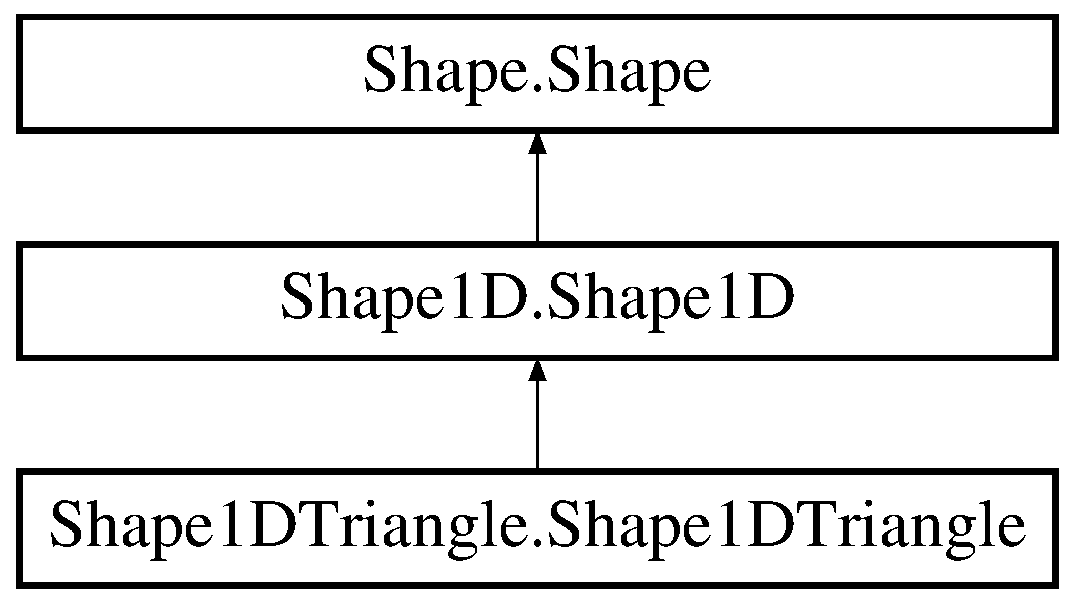
\includegraphics[height=3.000000cm]{classShape1D_1_1Shape1D}
\end{center}
\end{figure}
\subsection*{Additional Inherited Members}


\subsection{Detailed Description}
\begin{DoxyVerb}Documentation for Shape1D class
\end{DoxyVerb}
 

The documentation for this class was generated from the following file\-:\begin{DoxyCompactItemize}
\item 
Shape1\-D.\-py\end{DoxyCompactItemize}

\hypertarget{classShape1DTriangle_1_1Shape1DTriangle}{\section{Shape1\-D\-Triangle.\-Shape1\-D\-Triangle Class Reference}
\label{classShape1DTriangle_1_1Shape1DTriangle}\index{Shape1\-D\-Triangle.\-Shape1\-D\-Triangle@{Shape1\-D\-Triangle.\-Shape1\-D\-Triangle}}
}
Inheritance diagram for Shape1\-D\-Triangle.\-Shape1\-D\-Triangle\-:\begin{figure}[H]
\begin{center}
\leavevmode
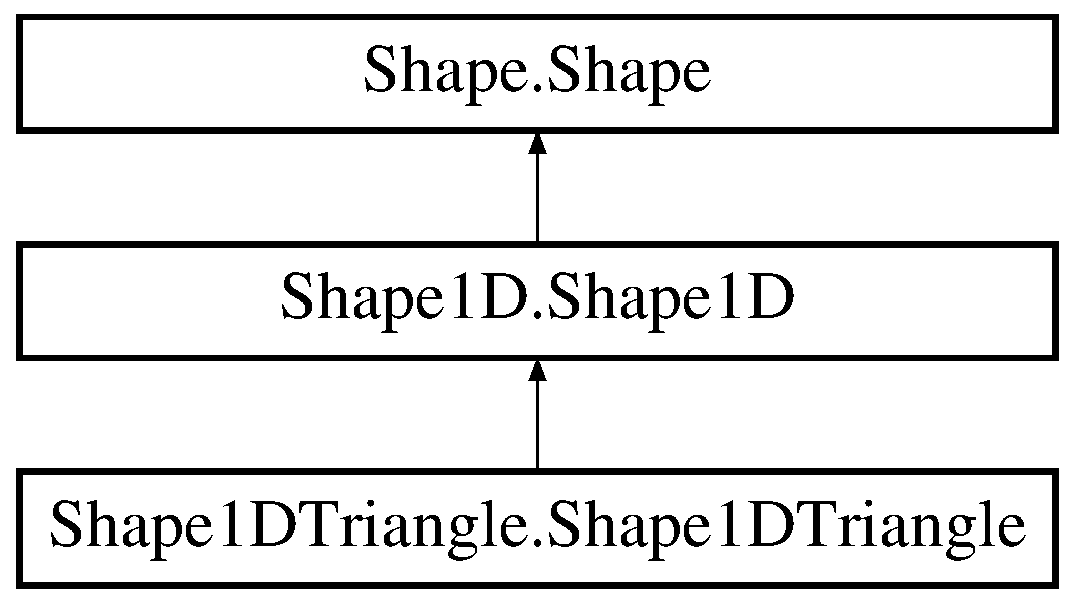
\includegraphics[height=3.000000cm]{classShape1DTriangle_1_1Shape1DTriangle}
\end{center}
\end{figure}
\subsection*{Public Member Functions}
\begin{DoxyCompactItemize}
\item 
def \hyperlink{classShape1DTriangle_1_1Shape1DTriangle_abb28fd4c5719c265e7230713150b0de2}{\-\_\-\-\_\-init\-\_\-\-\_\-}
\item 
def \hyperlink{classShape1DTriangle_1_1Shape1DTriangle_a38ee493cad6e07882bf1b4616fe44035}{get\-\_\-height}
\end{DoxyCompactItemize}


\subsection{Detailed Description}
\begin{DoxyVerb}Documentaiton for Shape1DTriangle class
\end{DoxyVerb}
 

\subsection{Constructor \& Destructor Documentation}
\hypertarget{classShape1DTriangle_1_1Shape1DTriangle_abb28fd4c5719c265e7230713150b0de2}{\index{Shape1\-D\-Triangle\-::\-Shape1\-D\-Triangle@{Shape1\-D\-Triangle\-::\-Shape1\-D\-Triangle}!\-\_\-\-\_\-init\-\_\-\-\_\-@{\-\_\-\-\_\-init\-\_\-\-\_\-}}
\index{\-\_\-\-\_\-init\-\_\-\-\_\-@{\-\_\-\-\_\-init\-\_\-\-\_\-}!Shape1DTriangle::Shape1DTriangle@{Shape1\-D\-Triangle\-::\-Shape1\-D\-Triangle}}
\subsubsection[{\-\_\-\-\_\-init\-\_\-\-\_\-}]{\setlength{\rightskip}{0pt plus 5cm}def Shape1\-D\-Triangle.\-Shape1\-D\-Triangle.\-\_\-\-\_\-init\-\_\-\-\_\- (
\begin{DoxyParamCaption}
\item[{}]{self, }
\item[{}]{size}
\end{DoxyParamCaption}
)}}\label{classShape1DTriangle_1_1Shape1DTriangle_abb28fd4c5719c265e7230713150b0de2}
\begin{DoxyVerb}The constructor
\end{DoxyVerb}
 

\subsection{Member Function Documentation}
\hypertarget{classShape1DTriangle_1_1Shape1DTriangle_a38ee493cad6e07882bf1b4616fe44035}{\index{Shape1\-D\-Triangle\-::\-Shape1\-D\-Triangle@{Shape1\-D\-Triangle\-::\-Shape1\-D\-Triangle}!get\-\_\-height@{get\-\_\-height}}
\index{get\-\_\-height@{get\-\_\-height}!Shape1DTriangle::Shape1DTriangle@{Shape1\-D\-Triangle\-::\-Shape1\-D\-Triangle}}
\subsubsection[{get\-\_\-height}]{\setlength{\rightskip}{0pt plus 5cm}def Shape1\-D\-Triangle.\-Shape1\-D\-Triangle.\-get\-\_\-height (
\begin{DoxyParamCaption}
\item[{}]{self, }
\item[{}]{position, }
\item[{}]{particle\-\_\-position}
\end{DoxyParamCaption}
)}}\label{classShape1DTriangle_1_1Shape1DTriangle_a38ee493cad6e07882bf1b4616fe44035}
\begin{DoxyVerb}Return the value of the shape function at a given function.
This function has to be overrided by the subclass.
\end{DoxyVerb}
 

The documentation for this class was generated from the following file\-:\begin{DoxyCompactItemize}
\item 
Shape1\-D\-Triangle.\-py\end{DoxyCompactItemize}

%--- End generated contents ---

% Index
\newpage
\phantomsection
\addcontentsline{toc}{part}{Index}
\printindex

\end{document}
